% !TEX root = 0_main.tex
\chapter{Private Function Evaluation}\label{chap:secproc}
Two-party Private Function SFE (PF-SFE) allows secure computation of a function $f_{Alice}(\cdot)$ held by one party (Alice) operating on another party's data $x_{Bob}$ (Bob) while both the data and the function are kept private.
This is in contrast to the usual setting of SFE where the function is known by both parties.
PF-SFE is especially useful when the function is proprietary or classified.

It is well known that PF-SFE can be reduced to regular SFE by securely evaluating a Universal Circuit (UC) \cite{sander1999non}.
UC is a circuit capable of simulating any circuit (function) $f(\cdot)$ given the description of $f(\cdot)$ as input \cite{Valiant76,KS08UC}.
More formally:
$$UC(f_{Alice}(\cdot),x_{Bob}) = f_{Alice}(x_{Bob}).$$
Secure evaluation of UC completely hides the functionality of $f(\cdot)$, including its topology.
Subsequent works have shown how to allow PF-SFE while avoiding the overhead of UCs \cite{KatzM11, MohasselS13}.

A UC is similar to a Universal Turing Machine (UTM) \cite{turing1936computable,herken1995universal} that receives a Turing machine description $f_{Alice}(\cdot)$ and applies it to the input data ($x_{Bob}$) on its tape \cite{davis2001engines}.
One party provides the machine description and the other one provides the initial data.
The output $f_{Alice}(x_{Bob})$ resides on the tape after the operation is completed.
A general purpose processor is a special realization of a UTM.
It receives a list of \emph{instructions} $f_{Alice}(\cdot)$ and applies them to the input data $x_{Bob}$ in memory.

\section{Arithmetic Logic Unit}
The core of conventional processors is the Arithmetic Logic Unit (ALU) which receives two \emph{operands} and an \emph{opcode} indicating the desired operation.
ALU supports an operation set consisting of operations like addition, multiplication, XOR, etc.
The ALU circuit consists of multiple sub-circuits for these operations and a MUX which selects one of their outputs.
Secure evaluation of an ALU, where the opcode comes from one party and operands come from the other party, keeps the operations private.
Thus, ALU can be thought of as an emulator of a simple UC in which the input function $f_{Alice}(\cdot)$ is limited to a single operation.

One can combine a number of ALUs to make a more comprehensive UC that can support functions consisting of multiple operations.
Unfortunately, this approach is not practical as the complexity of the circuit grows linearly with the number of operations.
On the other hand, in conventional processors, ALUs are combined with arrays of FFs, a.k.a., \emph{registers}, in order to store the intermediate values for supporting functions with arbitrarily large number of operations.
Since none of the earlier implementations of GC explicitly supported memory elements such as FFs, the ways to connect the feedback loop around the ALU were rather limited.
However, an explicit sequential description supported by \sys{} allows us to leverage conventional processor architectures.
Therefore, the \sys{} methodology not only provides a powerful method for generating compact circuits with a low overhead for SFE, but also paves the way for systematically building scalable sequential circuits that can be used for PF-SFE.

The idea of using an ALU or a \emph{universal next-instruction circuit} in the GC protocol can also be found in \cite{liu2014automating}.
The objective of that paper was improving efficiency of SFE where the function is known by both parties, unlike PF-SFE where the function is private.
Nonetheless, instead of ALU they eventually decided to use an \emph{instruction-specific circuit} which leaks information about the function but results in less effort for non-private function evaluation.

\section{Memory}
The processor accesses the memory while executing an instruction to read the instruction and data and write the data back.
If the memory is securely evaluated along with the processor, the access patterns must be also oblivious to both parties.
On the other hand, if the memory is not evaluated securely, the access patterns could be revealed that in turn could reveal information about the function to Bob and about the data to Alice.
For example, the instruction read pattern discloses the branching decisions in the function which may leak information about the data.
Because of \sys{} sequential methodology, the memory can be easily implemented using MUX and arrays of FFs.
Thus, it can be included in the processor circuit to be evaluated securely using the GC protocol.
However, inclusion of MUXs and FFs increases the operation time and communication linearly with respect to the memory size.

One alternative approach for hiding memory access patterns is the use of Oblivious Random-Access Machine (ORAM) protocols \cite{goldreich1996software} which allows oblivious load/store operations with amortized polylogarithmic overhead \cite{gordon2012secure,liu2014automating,LO13,gentry2014garbled}.
For the sake of simplicity, we do not use ORAM in this work.
However, one can simply connect our implementation of PF-SFE to an ORAM to benefit from its lower amortized complexity.
As another alternate, \cite{ZE13} showed that algorithms can sometimes be rewritten to use data structures such as stacks, queues, or associative maps for which they give compact circuit constructions of poly-logarithmic size.

\section{Secure Processor}
We assume Alice provides the private function $f_{Alice}(\cdot)$ and Bob provides private data~$x_{Bob}$.
At the end of the operation, only Bob learns the output $f_{Alice}(x_{Bob})$.
Note that we are not considering the case where both parties learn the output as that would allow Alice to learn Bob's private data with an identity function ($f\equiv I$).
The protocol is as follows:

\begin{enumerate}
\item
  Alice and Bob agree on an instruction set architecture (ISA), its implementation (i.e., the processor circuit), the maximum number of sequential cycles, and the configuration of data $x_{Bob}$ in the memory.
\item
  Alice compiles the function $f_{Alice}(\cdot)$ according to the ISA.
  Her input is the compiled binary of the function.
\item
  Bob prepares his input based on the agreed configuration to initialize the processor memory.
\item
  Using any secure GC framework, Alice garbles the processor circuit for the maximum number of sequential cycles and Bob, after receiving his inputs with OT, evaluates the garbled processor circuit for the same number of cycles.

\item
  Alice reveals the output types such that Bob learns the value of the output $f_{Alice}(x_{Bob})$ stored in memory.
  This needs to be done only for agreed memory locations containing the outputs such that Bob does not learn intermediate values in the memory.
\end{enumerate}

Because of secure evaluation using the GC protocol in Step 4, no information about values in the circuit will be leaked except the output.
Without knowing internal values in the processor circuit, none of the parties can distinguish instructions or memory access patterns.
In the following, we demonstrate an implementation of a processor supporting the MIPS (Microprocessor without Interlocked Pipeline Stages) ISA, as an example of a garbled processor for securely evaluating private functions.

\section{MIPS}\label{sec:mips}
MIPS is a text-book Reduced Instruction Set Computing (RISC) ISA \cite{kane1992mips}.
The RISC ISA consists of a small set of simplified assembly instructions in contrast to Complex Instruction Set Computing (CISC) (e.g., x86 ISA) which includes more complex multi-step instructions \cite{hennessy2012computer}.
We choose a RISC ISA processor instead of CISC for the following main reasons: (i) lower number of non-XOR gates, (ii) simple and straightforward implementation, and (iii) availability and diversity of open-source implementations.
Moreover, we choose a single-cycle MIPS architecture (i.e., one instruction per sequential cycle).
Other architectures (i.e, multi-cycle and pipelined) increase the performance of the processor by parallelization.
However, the GC protocol does not benefit from such low level parallelization.
The only important factor for GC is the total number of non-XORs which is smaller in the single-cycle MIPS.
We follow the Harvard Architecture which has distinct instruction memory (IM) and data memory (DM) in order to separate the parties' inputs.
IM is a Read-Only Memory (ROM) that stores Alice's instructions.
DM is a Random Access Memory (RAM) that is initialized with Bob's input.
The parties' inputs are connected to the initial signal inputs of FFs in the memories.
Bob's outputs are connected to the outputs of FFs in the specified address of DM.
The output address in DM is part of the agreed memory configuration.

\begin{figure*}[t!]
\centering
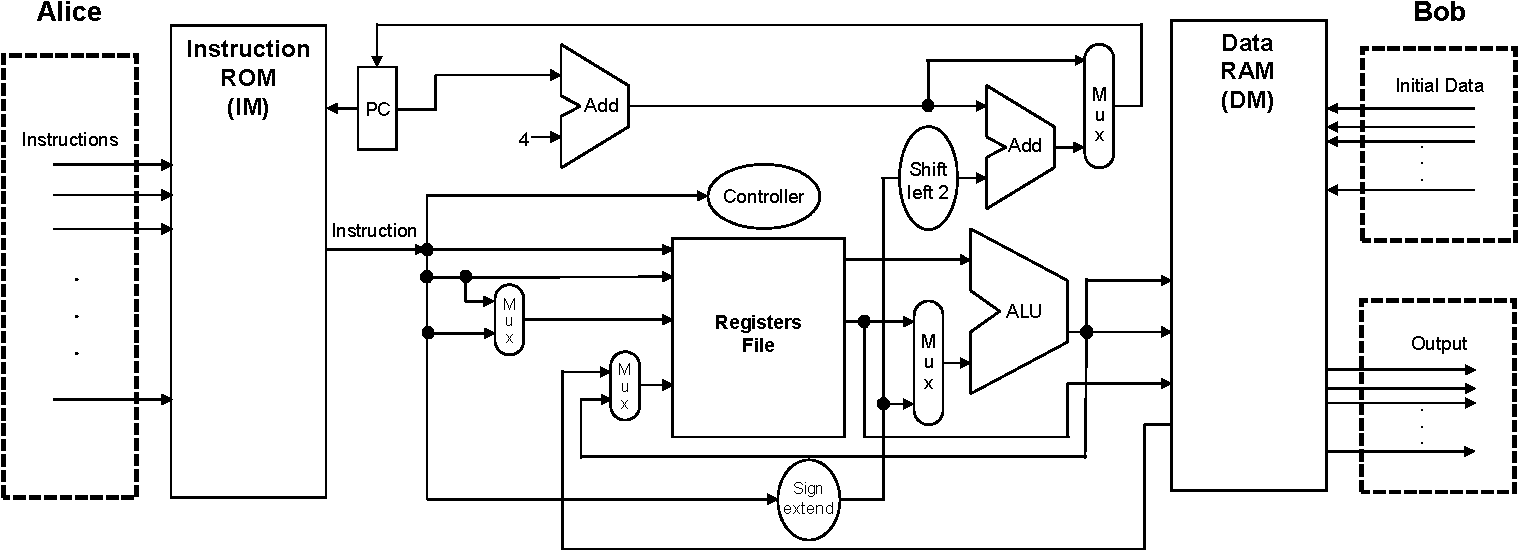
\includegraphics[width=0.95\textwidth]{mips-complex-crop.pdf}
\caption{Lite MIPS architecture.
  Alice's and Bob's inputs and the output are shown.}\label{figure:mips}
\end{figure*}

\fig{figure:mips} shows the overall architecture of our 32-bit MIPS processor.
It is based on the Plasma project in opencores \cite{rhoads2006plasma}.
We modified the circuit such that the instruction ROM (IM) and the data RAM (DM) are separated.
The original Plasma processor supports all the MIPS~I ISA except unaligned memory access.
In our implementation, we also omit division instructions because of their large overhead.
Any arbitrary C/C++ function can be easily compiled to MIPS~I assembly code using a cross-platform compiler e.g., GNU gcc.

In 32-bit MIPS, the program counter (\emph{PC}) is a 32-bit register (array of FFs) that points to the instruction being executed at the current cycle.
The instruction is fetched from IM based on the current PC value.
The \emph{controller} unit is responsible for setting signals to perform the instruction.
In 32-bit MIPS, the \emph{register file} consists of 32 registers of 32-bit each.
In each cycle, at most two registers can be read and at most one register can be written back.
ALU receives the read register(s) or a sign extended \emph{immediate} as operands.
ALU also receives an opcode from the controller unit.
The output of ALU will be either written back to the register file or fed to DM as an address for load/store.
The loaded data from DM is written back to the register file.
In each cycle, PC is incremented by 4 to point to the next instruction in IM or is changed according to a branch or jump instruction.
